\documentclass[extendedabs]{bmvc2k}

%\usepackage[table]{xcolor}
\usepackage{times}
\usepackage{epsfig}
\usepackage{graphicx}
\usepackage{amsmath}
\usepackage{amssymb}
\usepackage{subfigure}
\usepackage{multirow}
%% Enter your paper number here for the review copyu
%\bmvcreviewcopy{460}



%%%%%%%%%%%%%%%%%%%%%%%%%%%%%%%%%%
% AZ's macros
%%%%%%%%%%%%%%%%%%%%%%%%%%%%%%%%%%
% Stuff for doing vector.
\def\vec#1{\mathchoice%
        {\mbox{\boldmath $\displaystyle\bf#1$}}
        {\mbox{\boldmath $\textstyle\bf#1$}}
        {\mbox{\boldmath $\scriptstyle\bf#1$}}
        {\mbox{\boldmath $\scriptscriptstyle\bf#1$}}}
\def\v#1{\protect\vec #1}


% Stuff for doing matrix.
\def\mat#1{\mathchoice{\mbox{\boldmath$\displaystyle\tt#1$}}
        {\mbox{\boldmath$\textstyle\tt#1$}}
        {\mbox{\boldmath$\scriptstyle\tt#1$}}
        {\mbox{\boldmath$\scriptscriptstyle\tt#1$}}}
\def\m#1{\protect\mat #1}

\newcommand{\matx}[1]{{\m #1}}

\newcommand{\tr}{\mbox{$^{\top}$}}
\newcommand{\mtr}{\mbox{$^{-\top}$}}



%\title{Author Guidelines for the\\ British Machine Vision Conference}
%\title{Recognizing human actions in still images: a dataset, baselines and performance evaluation }
%\title{Recognizing human actions in still images: \\ comparison of bag-of-features and part-based approaches }
%\title{Recognizing human actions in still images: \\ a comparison of bag-of-features and part-based approaches }
%\title{Recognizing human actions in still images: \\ a comparison of bag-of-features and part-based representations}
\title{Recognizing human actions in still images: \\ a study of bag-of-features and part-based representations}
%\title{Recognizing human actions in still images: \\  bag-of-features or\\ part-based representation?}
%\title{Comparison of structured and unstructured representations for recognizing human actions in still images}

%\title{Recognizing human actions in still images: \\ a comparative study of bag-of-features and part-based approaches. }
%\title{Bag-of-features models for classification of human actions in still images}



% Enter the paper's authors in order
% \addauthor{Name}{email/homepage}{INSTITUTION_CODE}
\addauthor{Vincent Delaitre}{vincent.delaitre@ens-lyon.org}{1}
\addauthor{Ivan Laptev}{ivan.laptev@inria.fr}{2}
\addauthor{Josef Sivic}{josef.sivic@ens.fr}{2}

% Enter the institutions
% \addinstitution{Name\\Address}
\addinstitution{
\'Ecole Normale Sup\'erieure de Lyon\\
}
\addinstitution{
INRIA - Willow Project\\
%Laboratoire d'Informatique de l'Ecole Normale Superieure\\
Laboratoire d'Informatique\\
\'Ecole Normale Sup\'erieure\\
CNRS/ENS/INRIA (UMR 8548)\\
}

\runninghead{Delaitre, Laptev, Sivic}{Recognizing human actions in still images.}

% Any macro definitions you would like to include
% These are not defined in the style file, because they don't begin
% with \bmva, so they might conflict with the user's own macros.
% The \bmvaOneDot macro adds a full stop unless there is one in the
% text already.
\def\eg{\emph{e.g}\bmvaOneDot}
\def\Eg{\emph{E.g}\bmvaOneDot}
\def\etal{\emph{et al}\bmvaOneDot}

\newcommand{\red}[1]{{\em \small \color{red} #1}} % add
\definecolor{mygreen}{rgb}{0.0,0.6,0.1}
%\newcommand{\green}[1]{{\color{mygreen} #1}} %added
\newcommand{\green}[1]{#1} %added

\newcommand{\ok}[1]{{\small \scriptsize  \color{mygreen} #1}} %added
\newcommand{\bad}[1]{{\small \scriptsize  \color{red} #1}} %added


\newcommand{\secnspc}{\vspace*{-2mm}}       % -2
\newcommand{\subsecnspc}{\vspace*{-1.4mm}}  % -1.4
\newcommand{\parnspc}{\vspace*{-4.2mm}}     % -4.2
\newcommand{\capnspc}{\vspace*{-4mm}}       % -4

\newcommand{\tfs}{\small}   % tabular font size
\newcommand{\cfs}{\small}   % caption font size


%------------------------------------------------------------------------- 
% Document starts here
\begin{document}



\maketitle


Human actions represent essential content of many images. Recognizing human actions in still images will potentially provide useful meta-data to many applications such as indexing and search of large-scale image archives. Given the frequent interaction of people with objects (e.g. ``answer phone'') and scenes (e.g. ``walking around the corner''), human action recognition is also expected to help solving other related problems for still images such as object recognition or  scene layout estimation.

Recognition of human actions has mostly been explored in video. While the motion of people often provides discriminative cues for action classification, many actions such as the ones illustrated in Figure~\ref{fig:dataset} can be identified from single images. Moreover, several types of actions such as ``taking a photograph'' and ``reading a book'' are of static nature and may require recognition methods based on static cues only even if the video is available.

The goal of this work is to study recognition of common human actions represented in typical still images such as consumer photographs. This problem has received little attention in the past with the exception of a few related papers focused on actions in specific domains such as sports~\cite{Gupta09, FeiFei10b} and people playing musical instruments~\cite{FeiFei10a}.
%, or learning from still images to recognize actions in video. 
The proposed methods have mainly relied on the body pose as a cue for action recognition. While promising results have been demonstrated, typical action images such as the ones illustrated in Figure~\ref{fig:dataset} still present serious challenges for current body-pose estimation methods due  to heavy occlusions and significant changes in camera viewpoint. 

To deal with various types of actions in still images, we avoid explicit reasoning about body poses and investigate more general appearance-based classification methods. We study action recognition in typical consumer photographs and construct a new dataset with seven classes of actions in 968 images obtained from Flickr (Figure~\ref{fig:dataset}).

We investigate the performance of statistical bag-of-features (BOF) and spatial pyramid representations~\cite{Lazebnik06} combined with SVM classification. We examine a large set of parameters on the validation data and demonstrate consistent generalization of results to the test data. In particular, we investigate person-centric representations and study the influence of background/context information on action recognition. 
In addition to statistical methods, we also consider the structural part-based LSVM model of Felzenszwalb~\etal~\cite{Felzenszwalb09}. Figure~\ref{fig:backgnd_effect} illustrates results for both models individually as well for their combination. Figure~\ref{fig:hard_sample} illustrates the complementarity of BOF and LSVM models on a few sample images from our dataset.

Based on the comparative evaluation on the datasets of~\cite{Gupta09} and~\cite{FeiFei10a} (c.f. Table~\ref{tab:StateOfArt}), we finally demonstrate that the previous methods relying on explicit body-pose estimation can be significantly outperformed by more generic recognition methods investigated in this paper.

\bibliography{shortstrings,paper}

\vspace{-1mm}

%-------------------------------------------------------------------------------
\begin{figure}[ht]
%\centering
 \small
%\includegraphics[height=.5\linewidth]{figs/dataset.pdf}
%\includegraphics[height=.5\linewidth]{figs/images.png}
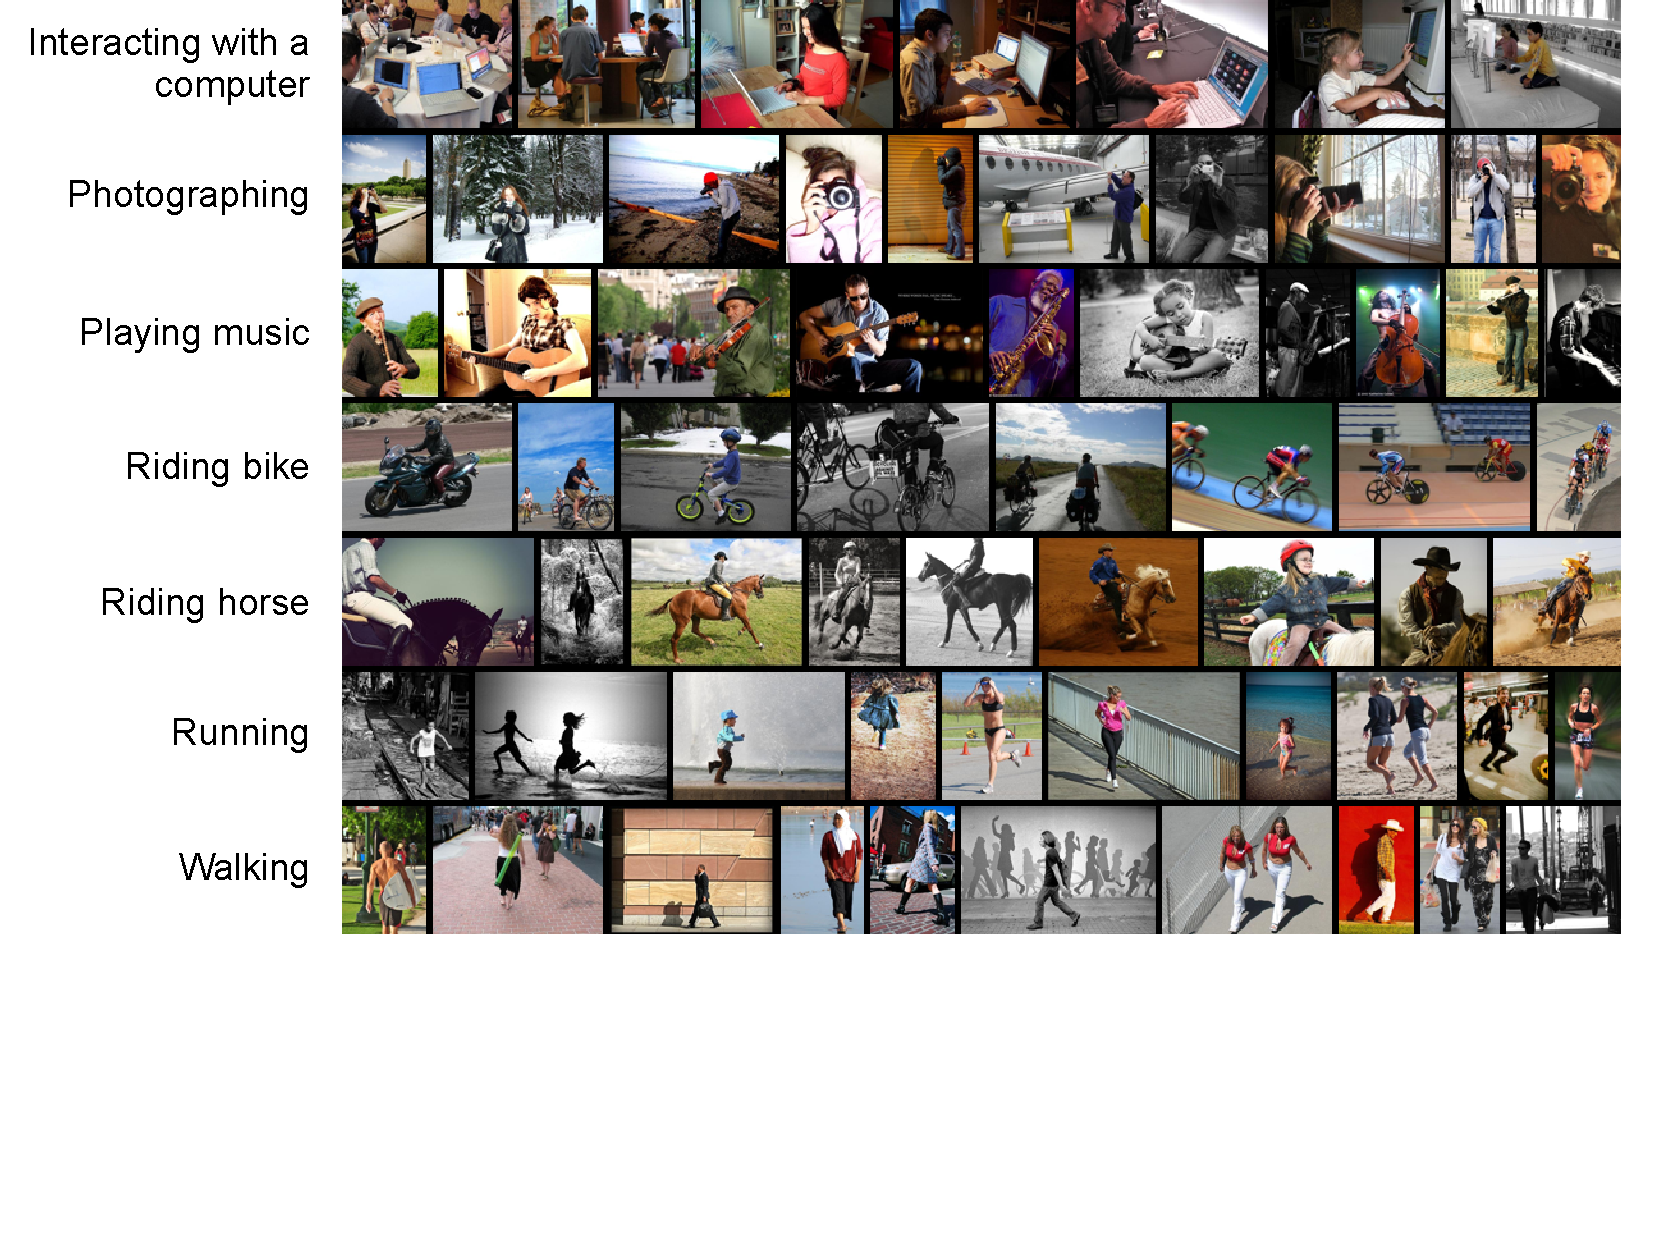
\includegraphics[width=.95\linewidth]{figs/my_dataset_cropped.pdf}
\vspace{-3mm}
\caption{\cfs Example images from our dataset with seven action classes collected from Flickr.
Note the natural and challenging variations in the camera view-point, clothing of people, occlusions, object appearance and scene layout present in consumer photographs.
%The manually annotated bounding boxes indicating the location of the person performing the action are overlaid in yellow. 
 %\red{*** Replace these Gupta images with examples of our images. Make images slightly bigger.}
 \normalsize
   }
 \label{fig:dataset}
\vspace{-2mm}
\end{figure}
%-------------------------------------------------------------------------------

%-------------------------------------------------------------------------------
\begin{figure}[ht]
\begin{center}
  \hspace{-.7cm}
  \begin{minipage}{0.53\linewidth}  
    \begin{tabular}{cc}
      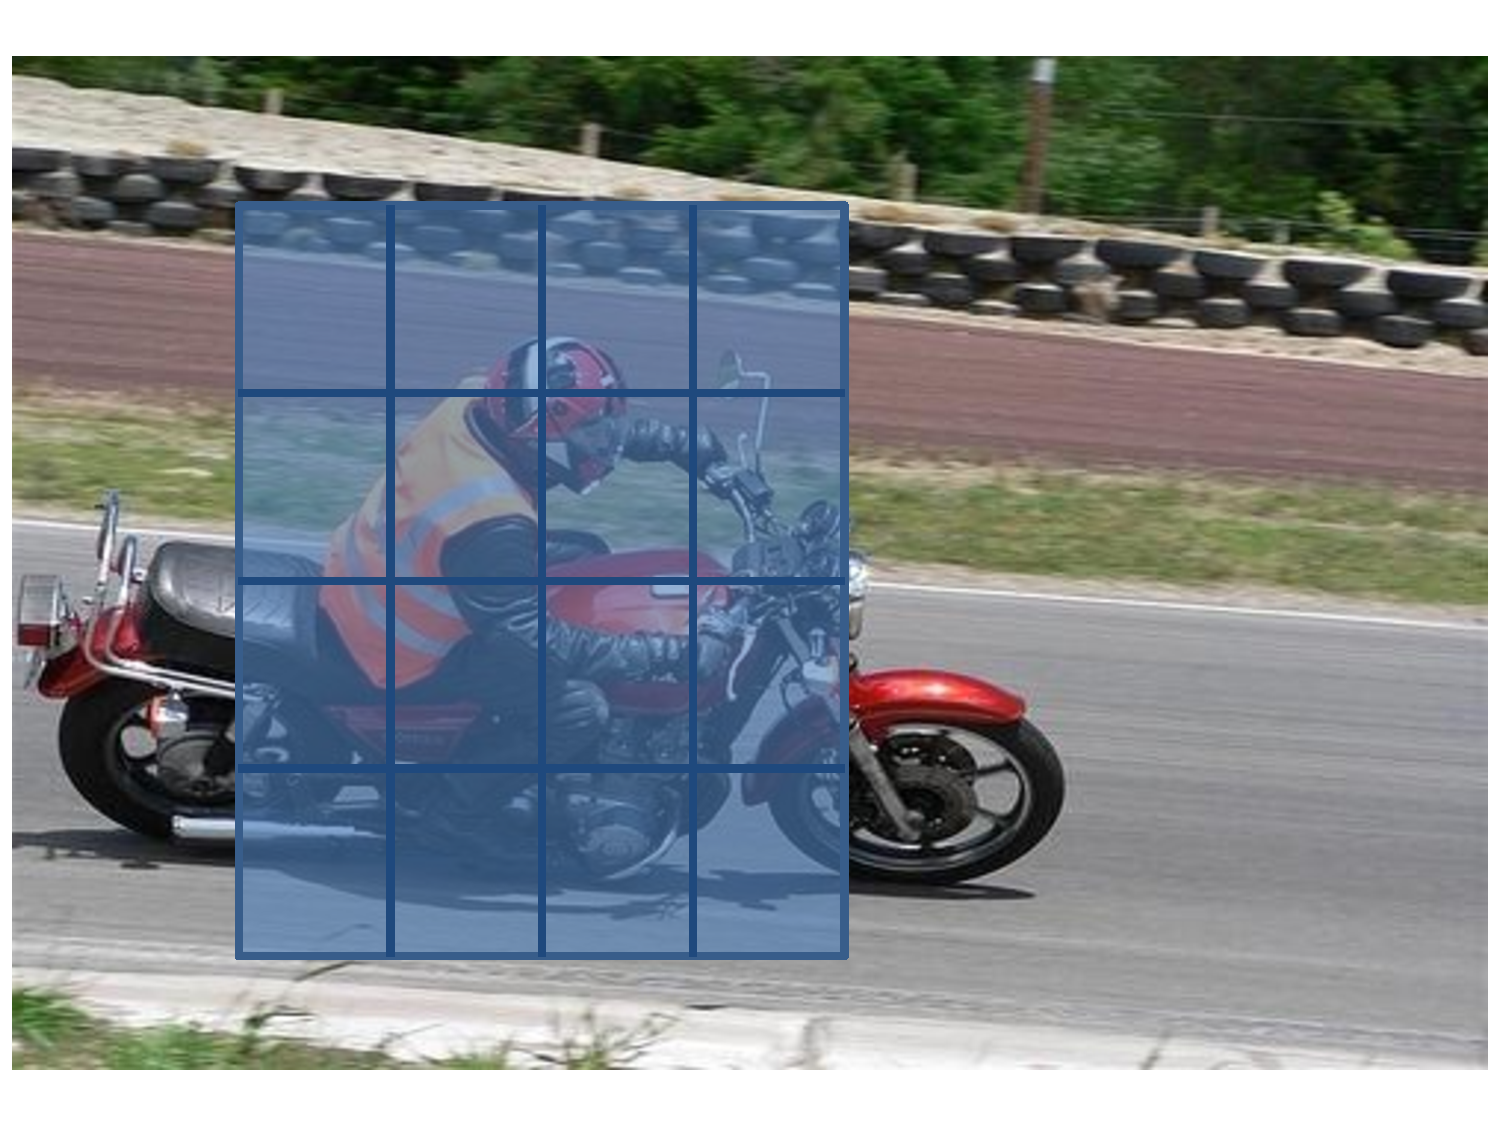
\includegraphics[width=0.42\linewidth]{figs/caseA.pdf} & \hspace{-.3cm}
      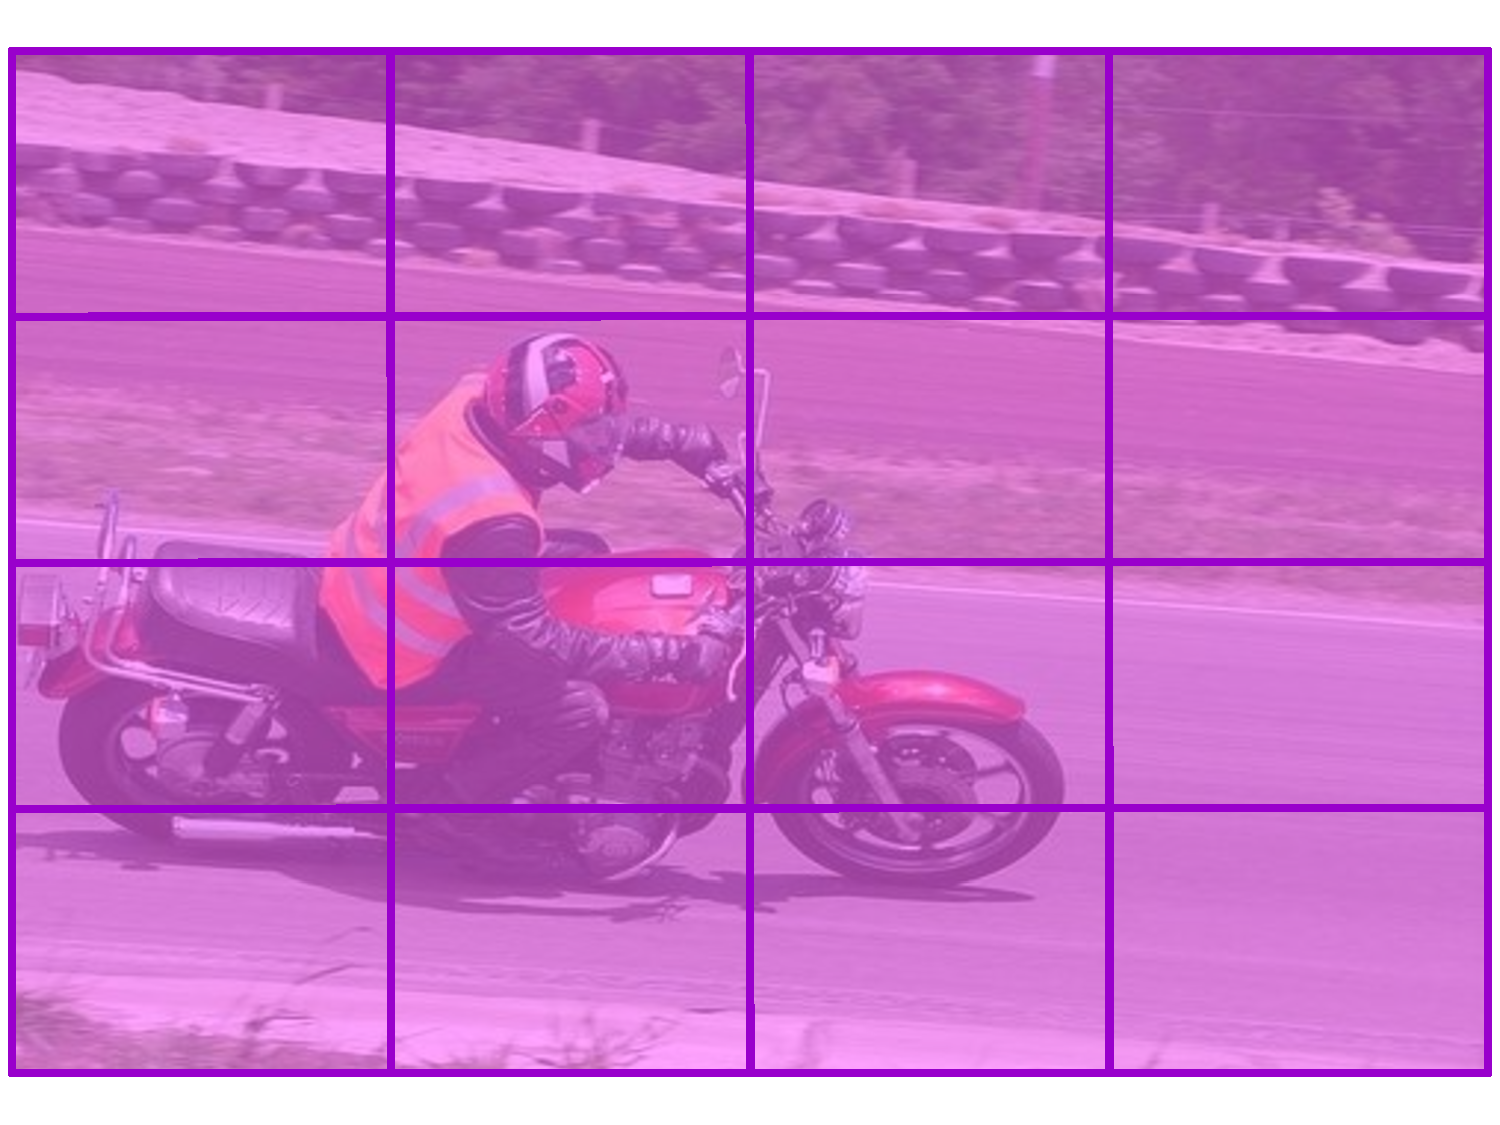
\includegraphics[width=0.42\linewidth]{figs/caseB.pdf}\vspace{-.2cm}\\
      (A)&(B)\vspace{-.1cm}\\
      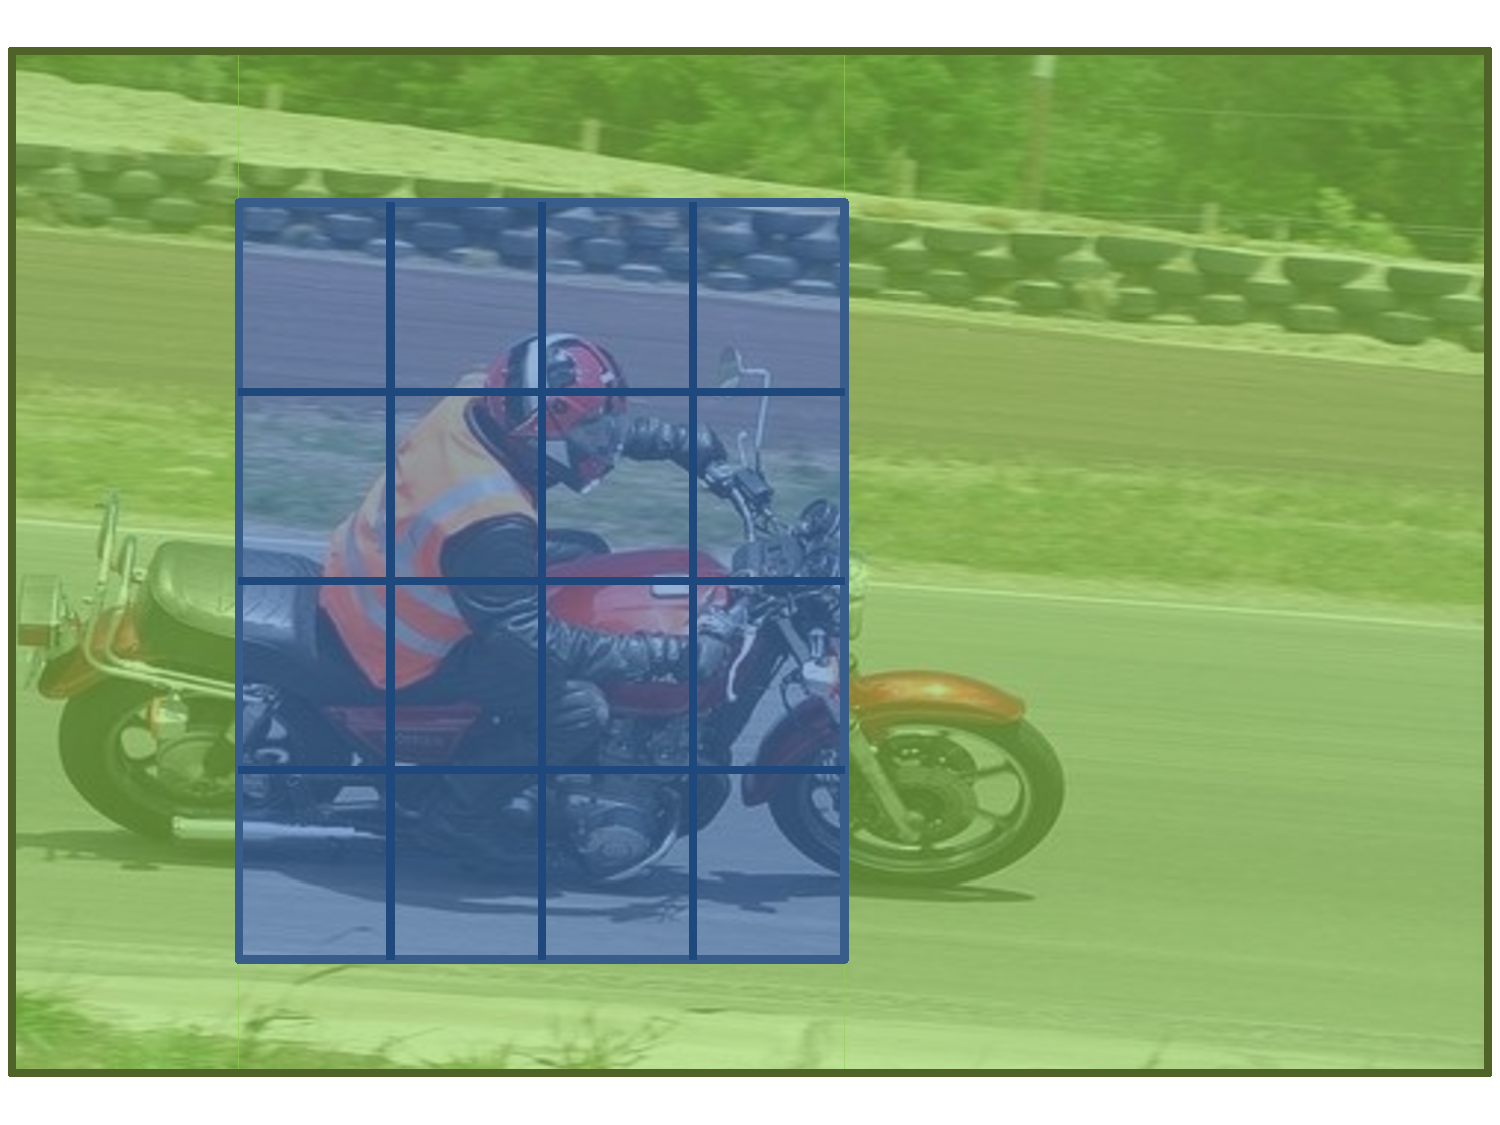
\includegraphics[width=0.42\linewidth]{figs/caseC1.pdf} & \hspace{-.3cm}
      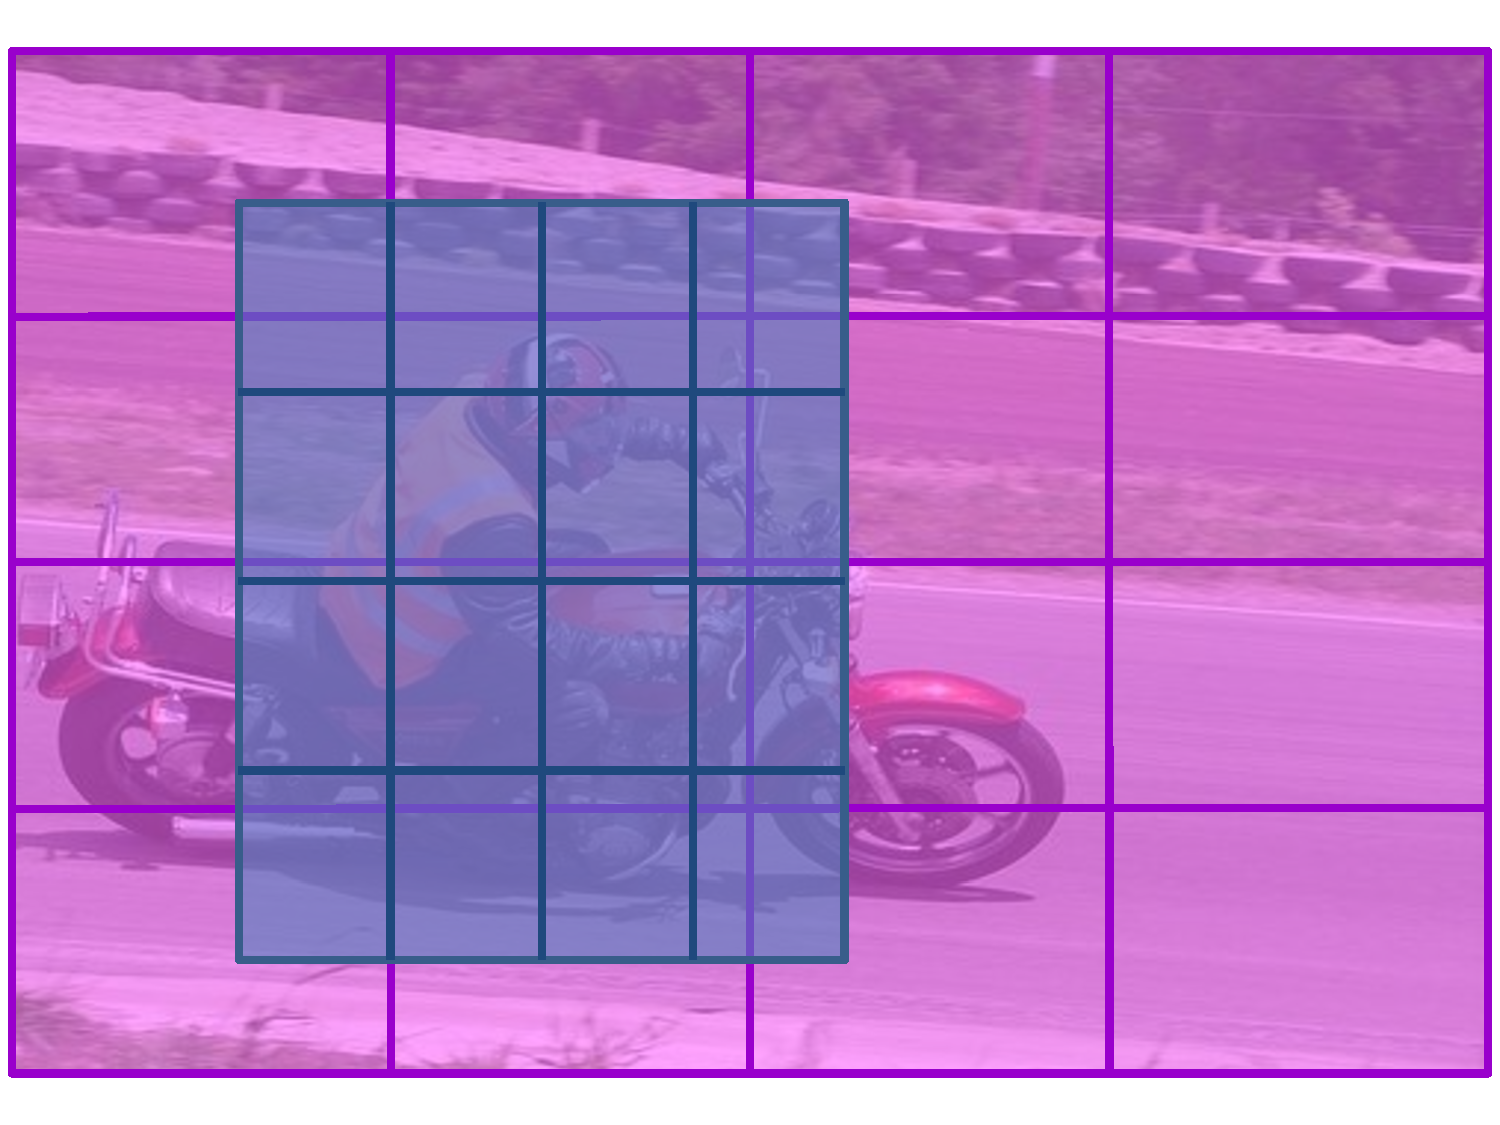
\includegraphics[width=0.42\linewidth]{figs/caseC2.pdf}\vspace{-.2cm}\\
      (C1)&(C2)\vspace{-.1cm}\\
    \end{tabular}
    %\subfigure[]{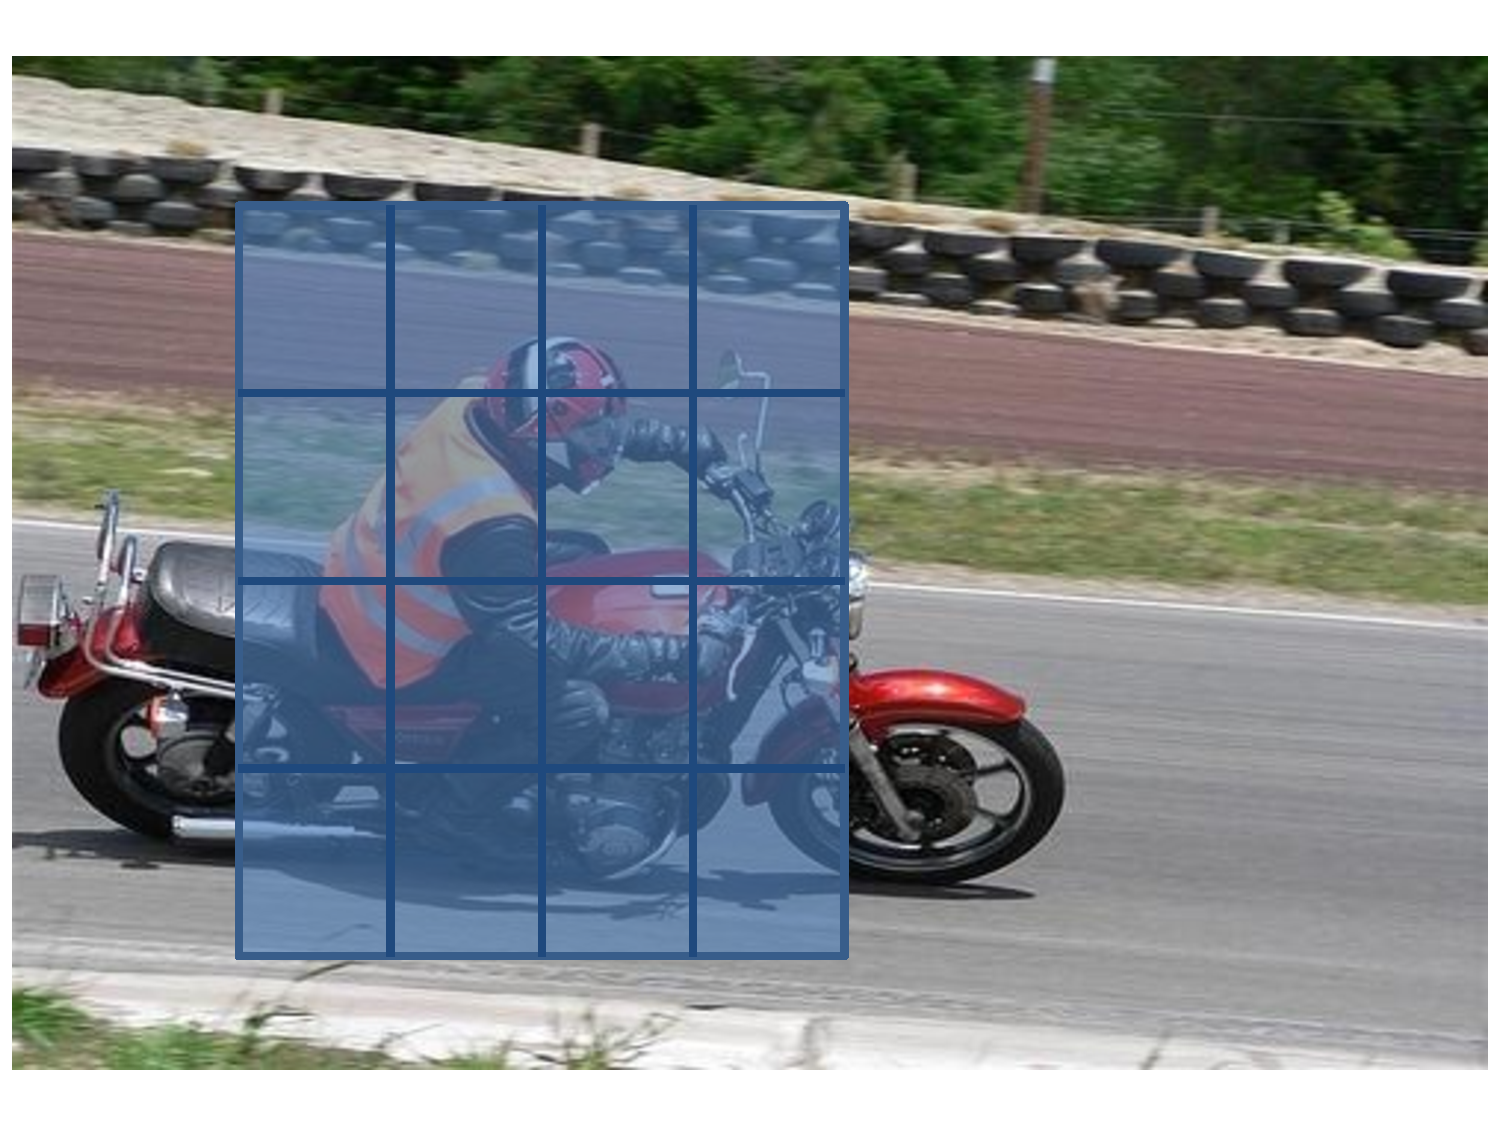
\includegraphics[width=0.45\linewidth]{figs/caseA.pdf}}\hfill
    %\subfigure[]{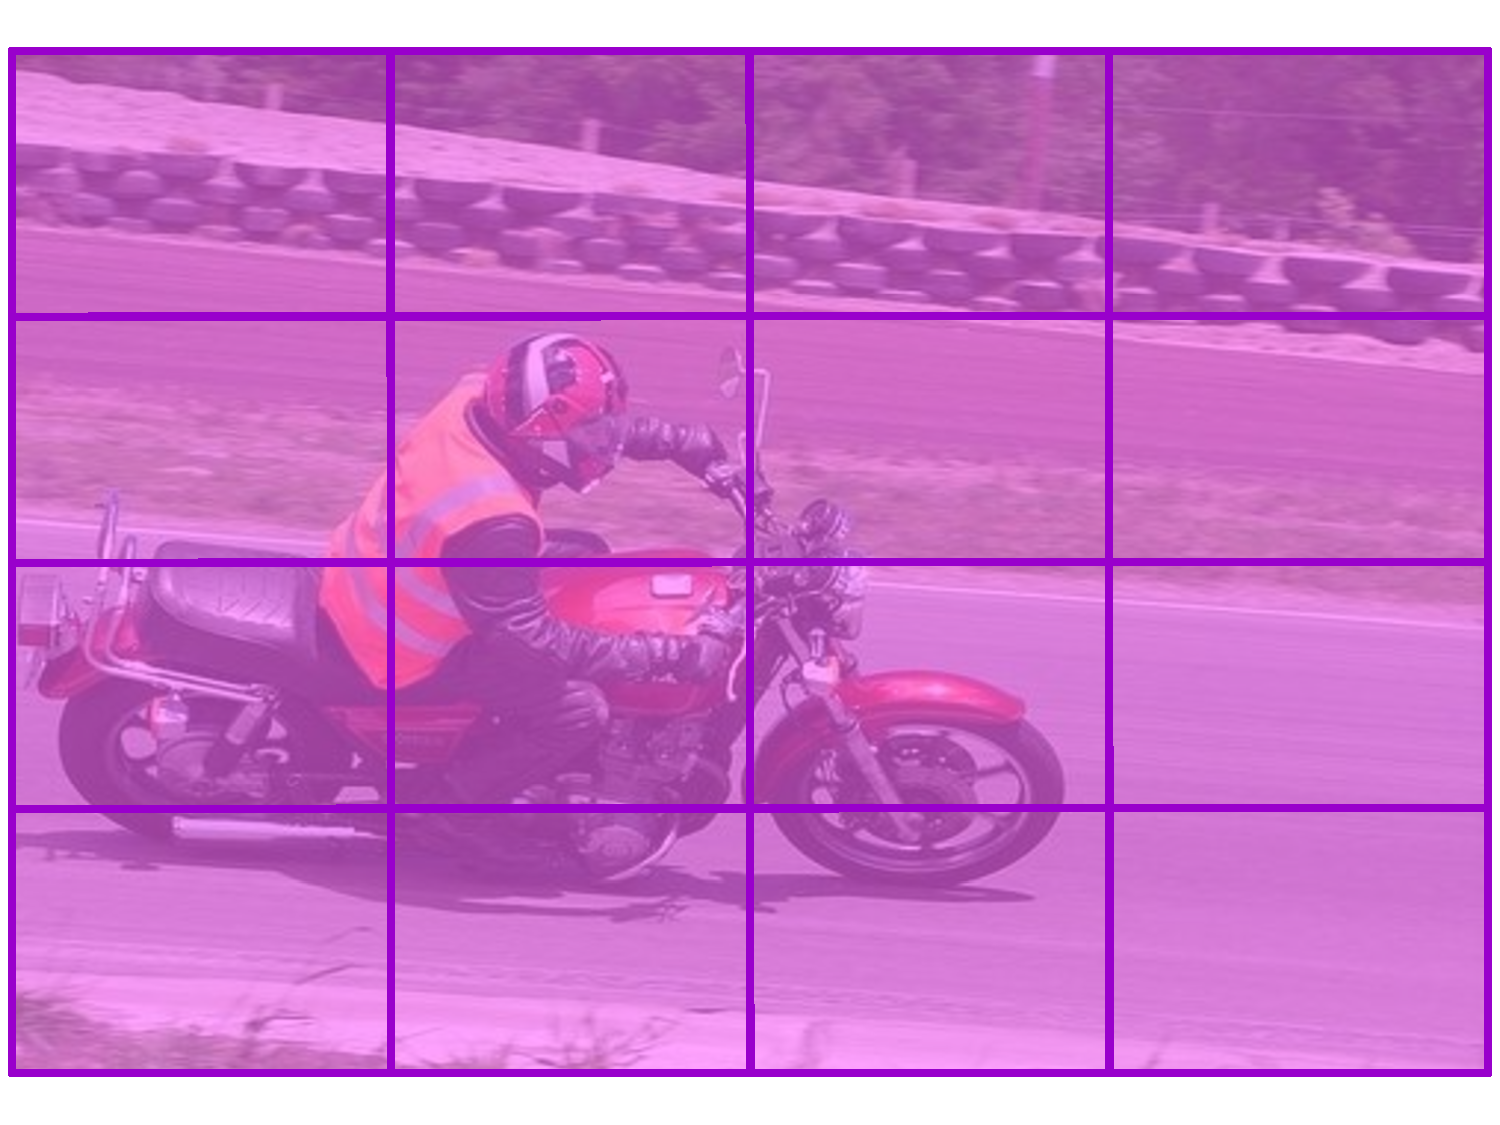
\includegraphics[width=0.45\linewidth]{figs/caseB.pdf}}\vspace{-4mm} \\ \vspace{-4mm}
    %\subfigure[]{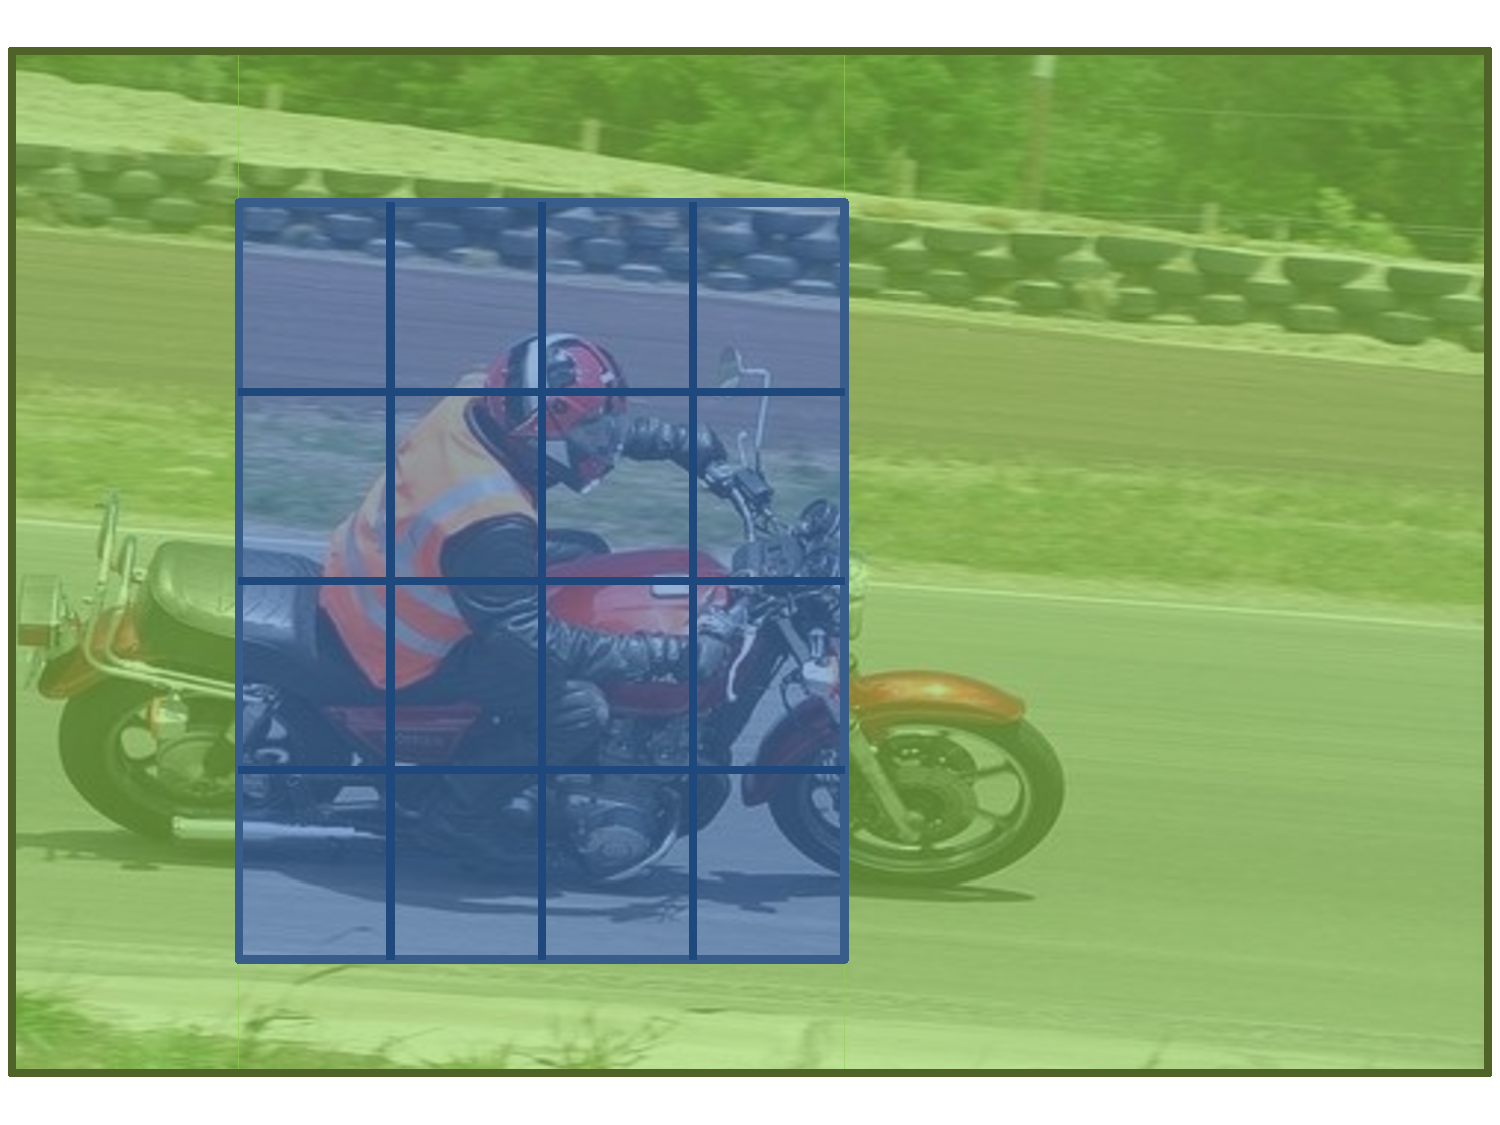
\includegraphics[width=0.45\linewidth]{figs/caseC1.pdf}}\hfill
    %\subfigure[]{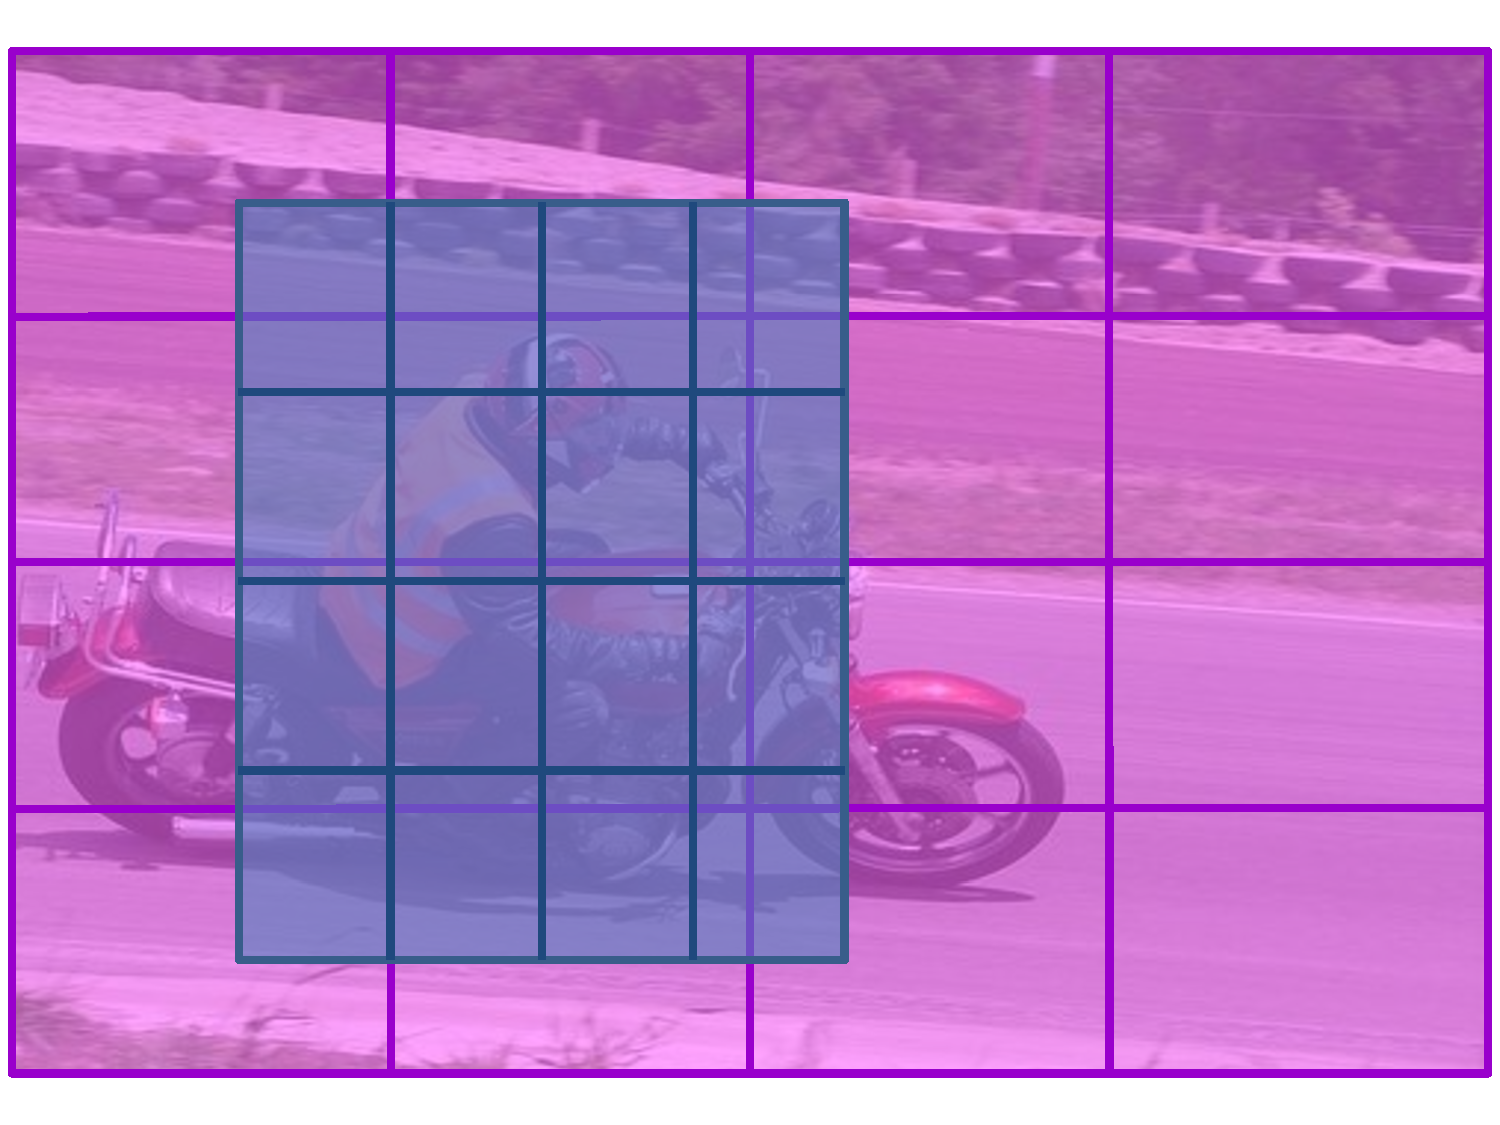
\includegraphics[width=0.45\linewidth]{figs/caseC2.pdf}}
  \end{minipage}
  \hspace{-.3cm}
  \begin{minipage}{0.45\linewidth}  
  %\vspace{4mm}
  %\subfigure[]{
    \begin{tabular}{|l||c|c|}
    \hline
    \tfs     &\tfs$~~~$mAP$~~~$& \tfs Accuracy  \\ \hline 
    \tfs BOF (A) &\tfs $61.48$ & \tfs $59.08$ \\ \hline 
    \tfs BOF (B) &\tfs $62.83$ & \tfs $60.24 $ \\ \hline 
    \tfs BOF (C1) &\tfs $63.96$ & \tfs $62.65$ \\ \hline 
    \tfs BOF (C2) &\tfs $70.43$ & \tfs $67.01$ \\ \hline \hline
    \tfs LSVM    & \tfs $55.12$ & \tfs $57.05$   \\ \hline \hline 
    \tfs LSVM +  & \multirow{2}*{\tfs ${\bf 72.16}$ } & \multirow{2}*{\tfs ${\bf 68.76}$} \\ 
    \tfs BOF (C2) & & \\ \hline     
    \end{tabular}
  %}
  \end{minipage}
\end{center}
\vspace{-2mm}
\caption{\cfs Different ways of integrating the background into the classifier: 
(A)~Spatial pyramid matching (SPM) on person only - limited use of background, 
(B)~SPM on the full image,
(C1)~2 channels: SPM on person + bag-of-features (BOF) over the rest of the image,
(C2)~2 channels: SPM on person + SPM over the full image.
Table on the right shows the performance of (A), (B), (C1) and (D) as well as the performance of LSVM and its combination with C2 (combination is obtained by adding classification scores).
\normalsize}
\label{fig:backgnd_effect}
\vspace{-2mm}
\end{figure}
%-------------------------------------------------------------------------------

%-------------------------------------------------------------------------------
\begin{figure}[ht]
\centering
%\rowcolors[]{1}{white}{gray!10}
\begin{tabular}{|c|c|c|c|}
\hline
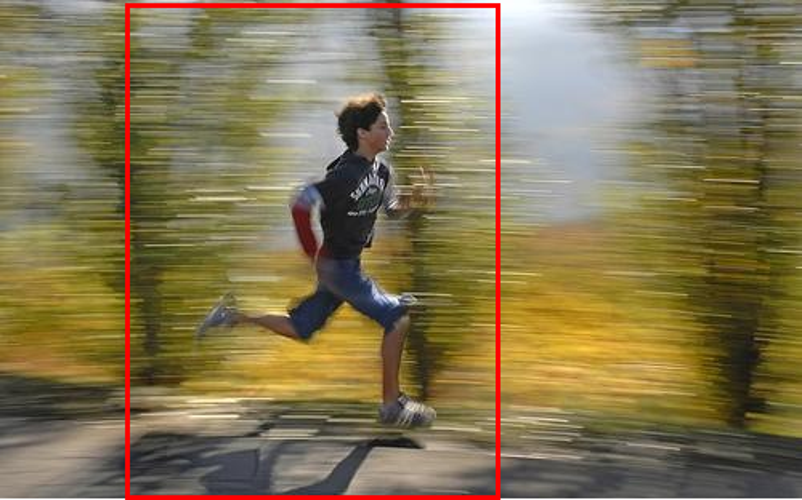
\includegraphics[height=.14\linewidth]{figs/misC2_RidingHorse_instead_Running_img0037.png}
&
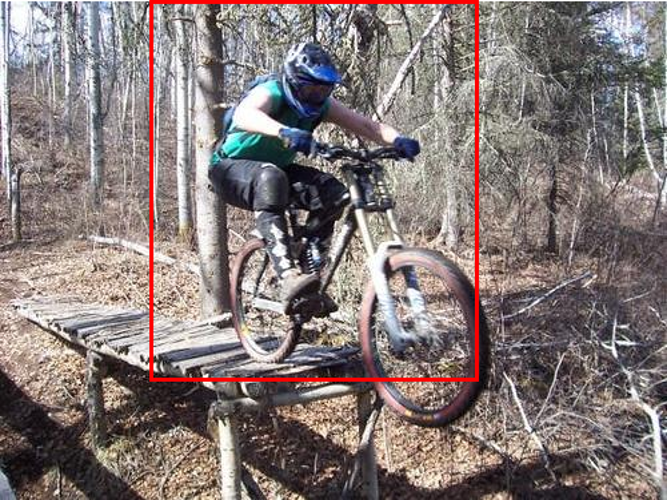
\includegraphics[height=.14\linewidth]{figs/misLSVM_RidingHorse_instead_RidingBike_img0192.png}
&
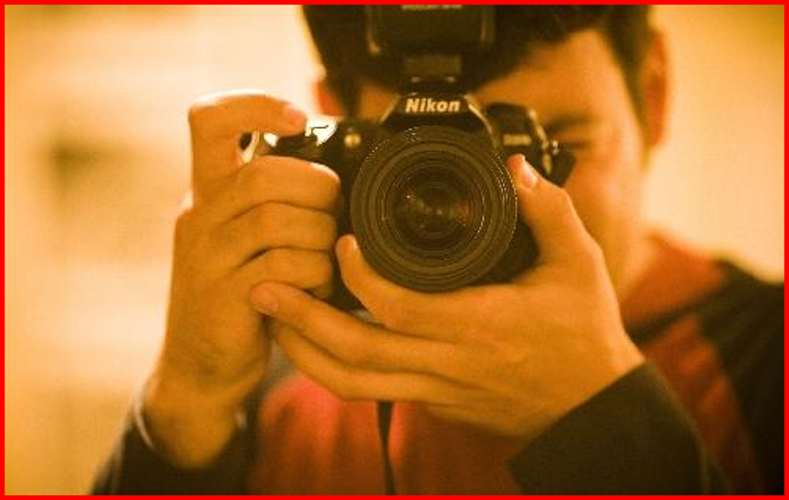
\includegraphics[height=.14\linewidth]{figs/misLSVM_PlayingMusic_instead_Photographing_img0009.png}
&

\includegraphics[height=.14\linewidth]{figs/misLSVMC2_PlayingMusic_instead_InteractingWithComputer_img0036.png}\\
\hline
 \scriptsize LSVM+BOF(d): | \ok{Running}         & \ok{RidingBike}   & \ok{Photographing}    & \bad{PlayingMusic} \\ \hline
 \scriptsize BOF (d):     | ~~~\bad{RidingHorse} & \ok{RidingBike}   & \bad{Inter. w/ comp.} & \bad{PlayingMusic} \\ \hline
 \scriptsize LSVM:        | ~~~\ok{Running}      & \bad{RidingHorse} & \bad{PlayingMusic}    & \bad{PlayingMusic} \\ \hline
\end{tabular}
\vspace{1mm}
\caption{\cfs Examples of challenging images and corresponding classifications. LSVM typically outperforms BOF on images with confusing (blurred, texture-less or
unusual) background, but with clearly visible pose of people. Similarly, the combined method improves LSVM
results mainly in cases where the camera viewpoint or the pose of the person are unusual.
\normalsize}
\label{fig:hard_sample}
\vspace{-2mm}
\end{figure}
%-------------------------------------------------------------------------------

%-------------------------------------------------------------------------------
\begin{table}[ht]
\centering
%\rowcolors[]{1}{white}{gray!10}
\begin{tabular}{|l||c|c||c|c||c|c|}
\hline
                        & \multicolumn{2}{c||}{Gupta \etal}  &\multicolumn{4}{c|}{Yao and Fei-Fei \cite{FeiFei10a}}     \\ \cline{4-7}
\multirow{-2}*{Dataset} & \multicolumn{2}{c||}{\cite{Gupta09}}                             &\multicolumn{2}{c||}{Task 1} &\multicolumn{2}{c|}{Task 2}  \\ \hline
Method  			                               & mAP             & Acc.           & mAP               & Acc.         & mAP               & Acc.                \\ \hline \hline
Gupta~\etal	                 & --         	   & $78.7$         & --                & --           & --                & --                  \\ \hline 
Yao and Fei-Fei                              & --	             & $83.3$         & --                & $65.7$       & --                & $80.9$              \\ \hline 
BOF (b)       		 	                         & $91.3$	         & ${\bf 85.0}$   & $76.9$            & $71.7$       & $87.7$            & $83.7$              \\ \hline 
LSVM 			  		                             & $77.2$          & $ 73.3 $       & $53.6$            & $67.6$       & $82.2$            & $82.9$              \\ \hline 
LSVM + BOF (b)	      	                     & ${\bf 91.6}$    & $ {\bf 85.0}$  & ${\bf 77.8}$      & ${\bf 75.1}$ & ${\bf 90.5}$      & ${\bf 84.9}$        \\ \hline 
\end{tabular}
\vspace{1mm}
\caption{\cfs Comparison with the methods of Gupta~\etal.~\cite{Gupta09} and of Yao and Fei-Fei \cite{FeiFei10a, FeiFei10b} on their datasets. `Task 1' is the 7-class
classification problem and `Task 2' is the PPMI+ vs PPMI- (person playing music) problem (see \cite{FeiFei10a} for details).\normalsize}
\label{tab:StateOfArt}
\end{table}
%-------------------------------------------------------------------------------

\end{document}
